\icode{E-MD-CA-L3-261111-001}
如图所示，质量为\(M =\) \,\qty{2}{kg}的木板\(B\)在光滑的地面上，在\(t = 0\)时刻其速度为\(v_2 =\) \,\qty{8}{m/s}，此时一质量为\(m =\) \,\qty{1}{kg}的物块\(A\) 以\(v_1 =\) \qty{4}{m/s}的速度从木板右端冲上木板，已知木板与物块间的动摩擦因数为\(\mu = 0.2\)，最大静摩擦力等于滑动摩擦力，且物块始终在木板上。取\(g =\) \,\qty{10}{m/s^2}，求木板的最小长度。

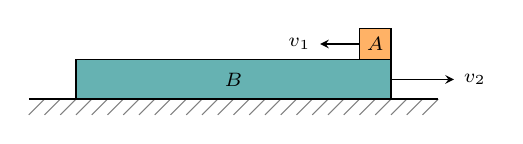
\begin{tikzpicture}[>=stealth,font=\scriptsize]
	\draw[fill=teal!60] (0,0) rectangle(4,.5)node[midway]{\(B\)};
	\draw[fill=orange!60] (4,.5) rectangle(3.6,.9)node[midway]{\(A\)};
	\draw[->] (4,.25)--++(.8,0)node[right]{\(v_2\)};
	\draw[->] (3.6,.7)--++(-.5,0)node[left]{\(v_1\)};
	\foreach \x in {-.6,-.4,...,4.6}
		\draw[gray] (\x,-.2)--++(.2,.2);
	\draw[thick] (-.6,0)--(4.6,0);
\end{tikzpicture}
\begin{answer}
	\qty{24}{m}\qquad 提示：
\end{answer}